日本と開発途上国との国際科学技術協力の強化や地球規模課題の解決、科学技術水準の
向上につながる新たな知見や技術の獲得等を目的とした地球規模課題対応国際科学技術協
力プログラム(SATREPS, Science and Technology Research Partnership for Sustainable
Development )のプロジェクトの1つに、ULAT(Understanding Lightning and Thunderstorms Project)
がある。ULATは東南アジアを中心に大規模な災害を引き起こしている雷雨や台風の高精
度な活動把握や予測を目的としたプロジェクトである。このプロジェクトにて、我々の研究
グループはP-POTEKAと呼ばれる自動気象観測装置(図\ref{fig:poteka-aws})を用いてマニ
ラ首都圏を中心にフィリピン全土をカバーする35カ所の雷・気象観測網(図\ref{fig:poteka-distribution-map})
を構築した。世界的にも類を見ないほどの高密度観測網であり、大規模な災害を引き起こす
雷雨や台風による降雨やそれに伴って変化する気温や湿度などの気象データを1分の時間解
像度で観測することができる。
P-POTEKAから得られるデータを表\ref{tb:poteka-observation-parameters}に示す。本研究では
時間雨量・気温・湿度、風向と風速から計算される東西/南北風成分のデータを用いた。
表\ref{tb:poteka-observation-parameters}の降水量は1分間の降水量を示す。過去60分間の降
水量を積算した時間雨量を降雨データとして用いた。

\begin{figure}[H]
\begin{center}
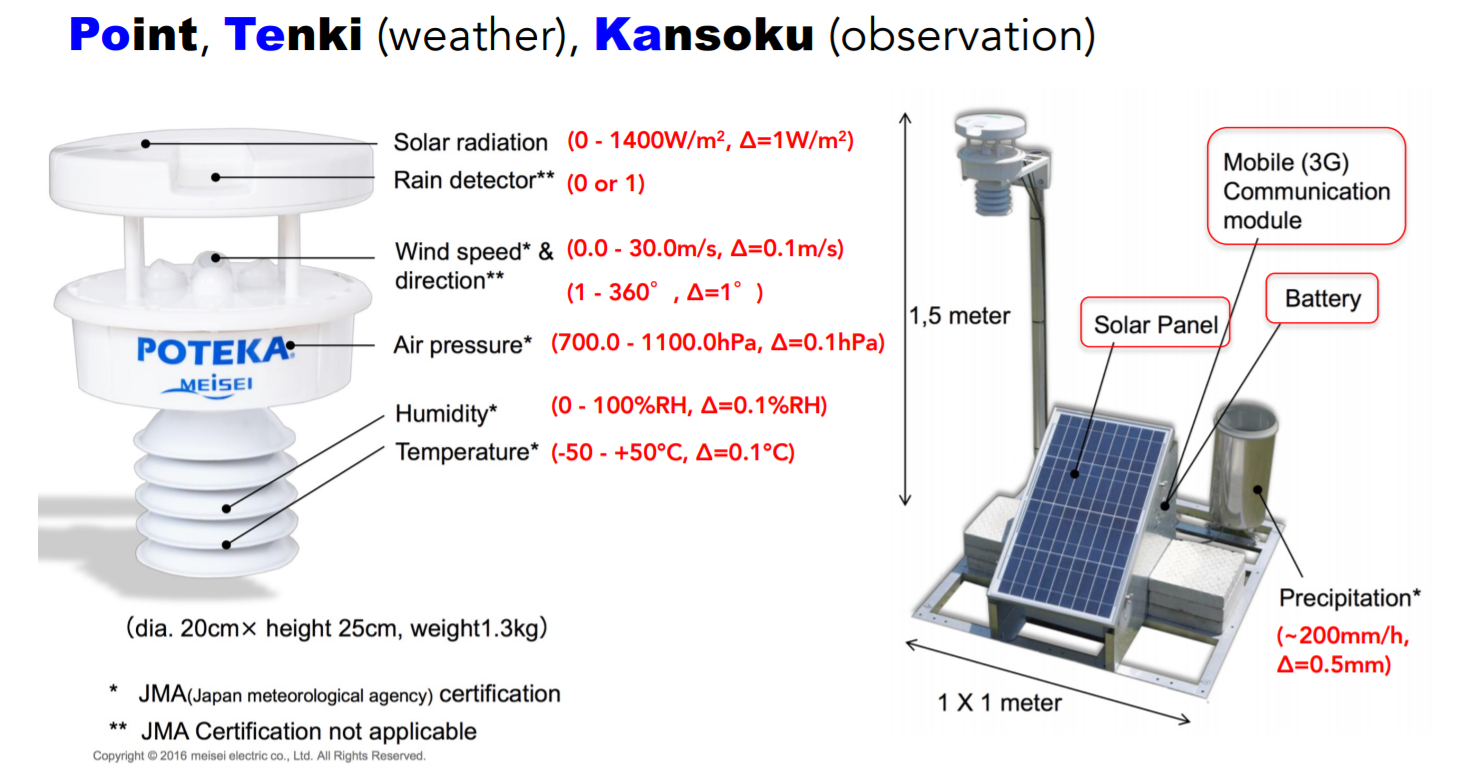
\includegraphics[width=0.9\linewidth]{fig/methodologies/poteka-aws.png}
\captionsetup{width=0.9\linewidth}
\caption{P-POTEKA観測装置。左図は気象センサを搭載した部分で、各部分で観測している気象データを示す。右図は観測装置全体。}
\label{fig:poteka-aws}
\end{center}
\end{figure}

\begin{figure}[H]
\begin{center}
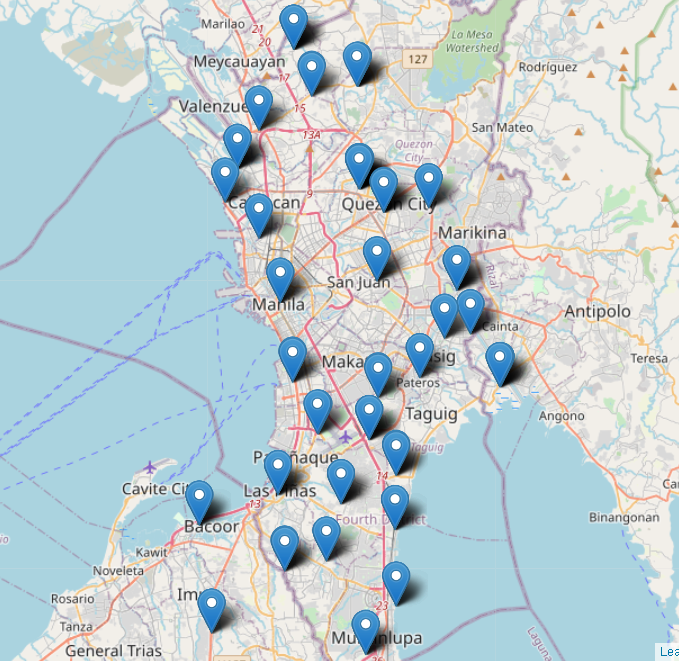
\includegraphics[width=0.8\linewidth]{fig/methodologies/poteka-distribution-map.png}
\captionsetup{width=0.8\linewidth}
\caption{マニラ首都圏のP-POTEKA分布図。}
\label{fig:poteka-distribution-map}
\end{center}
\end{figure}


\begin{table}[h]
\caption{P-POTEKAが観測する気象データ一覧。}
\label{tb:poteka-observation-parameters}
\centering
\begin{tabular}{cccc}
\hline
データ名[単位] & 最小値 & 最大値 & 解像度 \\
\hline \hline
日射[\si{W/m^{2}}] & 0 & 1400 & 1 \\
感雨 & 0 & 1 & 1 \\
風速[\si{m/s}] & 0 & 30 & 0.1 \\
風向[\si{\degree}] & 1 & 360 & 1 \\
気圧[\si{hPa}] & 700 & 1100 & 0.1 \\
湿度[\si{\%RH}] & 0 & 100 & 0.1 \\
気温[\si{\degreeCelsius}] & -50 & 50 & 0.1 \\
降水量[\si{mm}] & 0 & 200 & 0.5 \\
\hline
\end{tabular}
\end{table}

